Figure \ref{fig:trunk-cnf-reps}} shows the confusion matrix summarizing the classifications of the individual repetitions made by the ensemble presented in Table \ref{tab:ensemble-models} and Appendix \ref{}.
Each entry in the matrix is the mean along with the standard deviation for models from the 10 folds. Figures \ref{fig:trunk-cnf-comb}, \ref{fig:trunk-cnf-comb-th} shows the corresponding matrices for the combined scores, with and without the threshold suggested in \ref{sec:met-combined}.
These results are also summarized as accuracy and f1 scores in Table \ref{tab:trunk-results}. This table also shows the model performance performs for the data with different label certainty. Histograms for these metrics are shown in Figure \ref{fig:trunk-hist-results} along with the corresponding metrics for the individual models in the ensemble (high precision models are not shown as they only predict one label).

\begin{table}
  \centering
  \caption{Results of the ensemble for the trunk POE. Rep., Comb., and Thresh. represents the results for the repetitions, combinations, and combinations with thresholds respectively. The Certainties columns shows the results making up the Comb. column, but for the certainty levels of the expert labeling the data. These range from certain (1) to uncertain (3), n shows how many datapoints each category contains. All results are the mean from the 10 folds $\pm$ the corresponding standard deviations.}
  \label{tab:trunk-results}
  \small
  \begin{tabu}[c]{|c|c|c|c||c|c|c|}
    \hline
    % & \multirow21}{*}{Repetitions} & \multirow{2}{*}{Combinations} & \multirow{2}{*}{Thresholds} &  \multirow{2}{*}\multicolumn{3}{c}{Certainties}\\
    & \multirow{2}{*}{\textbf{Rep.}} & \multirow{2}{*}{\textbf{Comb.}} & \multirow{2}{*}{\textbf{Thresh.}} & \multicolumn{3}{c|}{\textbf{Certainties}}\\ \cline{5-7}
    & & & &1(n=15)&2(n=6)&3(n=1)\\ \hline
    Accuracy (\%) &73.7$\pm$4.5&75.0$\pm$7.9&\textbf{80.0$\pm$7.8}&\textbf{81.3$\pm$7.1}&56.7$\pm$15.2&90.0$\pm$30.0\\ \hline
    F1 score (\%) &73.1$\pm$3.4&75.0$\pm$5.8&\textbf{79.9$\pm$8.9}&\textbf{80.4$\pm$7.1}&25.8$\pm$6.3&90.0$\pm$30.0\\ \hline

  \end{tabu}
\end{table}

\begin{figure}
  \centering
  \begin{subfigure}[t]{0.48\textwidth}
      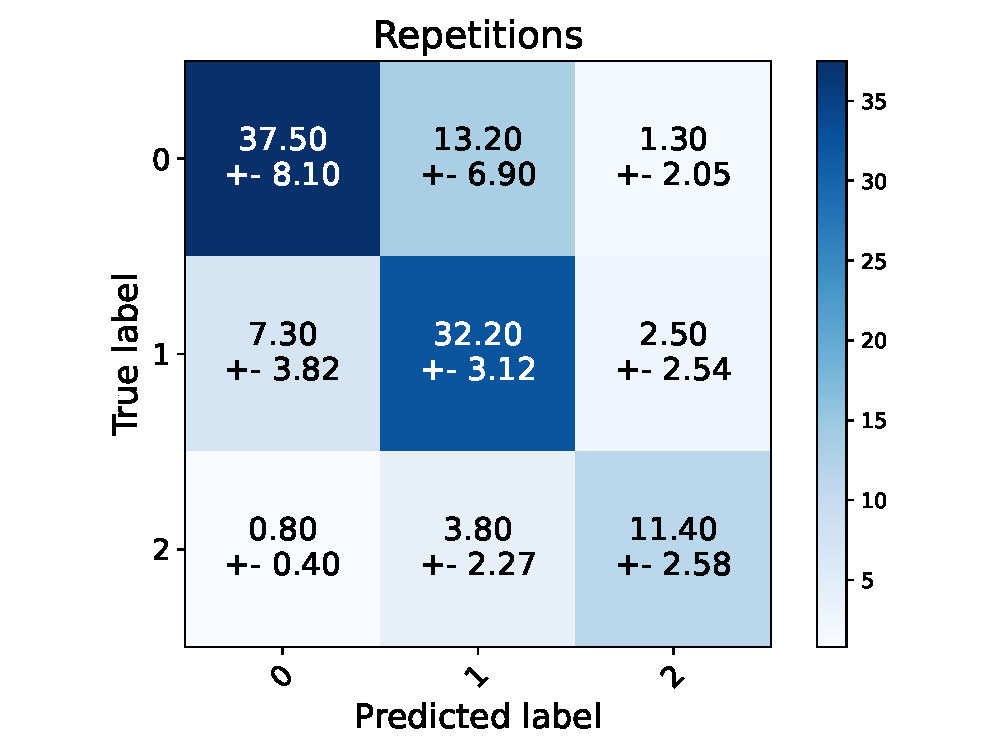
\includegraphics[width=\textwidth]{files/figs/res/trunk/cnf-reps.eps}
      \caption{}
      \label{fig:trunk-cnf-reps}
  \end{subfigure}
  ~
  \begin{subfigure}[t]{0.48\textwidth}
      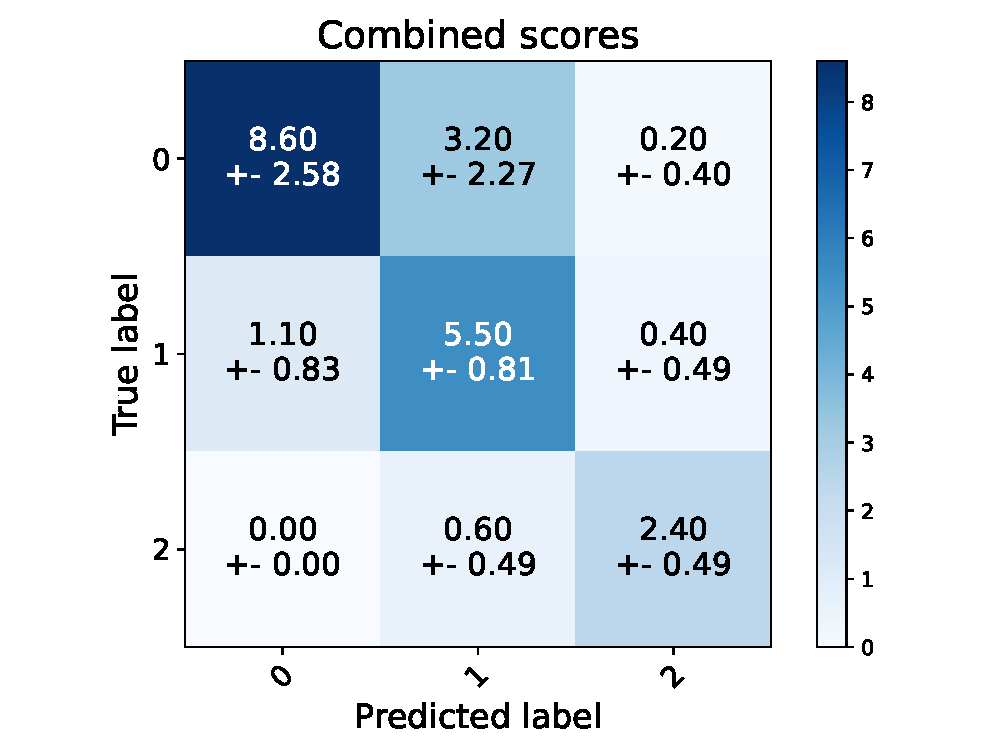
\includegraphics[width=\textwidth]{files/figs/res/trunk/cnf-combined.eps}
      \caption{}
      \label{fig:trunk-cnf-comb}
  \end{subfigure}

  \begin{subfigure}[t]{0.48\textwidth}
      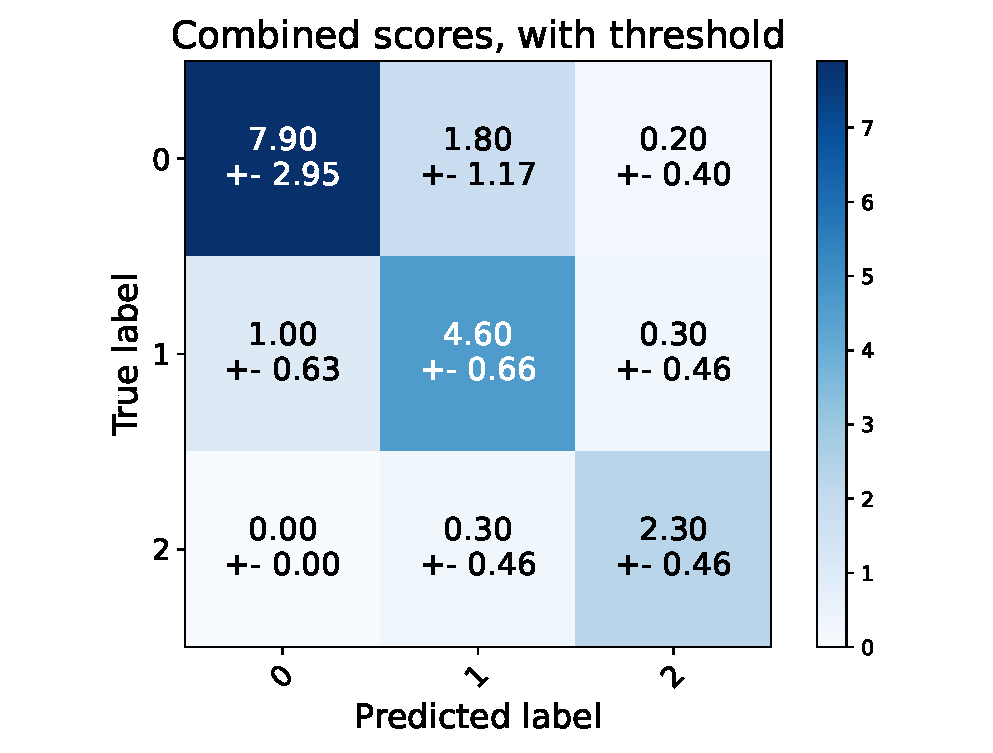
\includegraphics[width=\textwidth]{files/figs/res/trunk/cnf-combined-th.eps}
      \caption{}
      \label{fig:trunk-cnf-comb-th}
  \end{subfigure}
  \caption{Confusion matrices for the trunk classification on the test set. The entries in the matrices shows the mean and standard deviation of the 10 ensembles trained in the cross validation. Classification of the individual repetitions is shown in (a), the combined score for the sequences of 5 repetitions is shown in (b). (c) shows the combined score with the threshold suggested in Section \ref{sec:met-combined}, i.e. all scores with a predicted probability higher than 0.4.}
  \label{fig:trunk-cnfs}
\end{figure}

From Figure \ref{fig:trunk-cnfs} it is clear that the majority of misclassifications are between the classes 0 and 1. This is a natural effect of there being more 0s and 1s than 2s in the test set. However, asking the experts working with this assessment system these classes are generally the ones difficult to tell apart. Another sign that the model to some extent aligns with the assessments made by the human is the better performance for the sequences where the human expert were certain about the class, seen in Table \ref{tab:trunk-results}.

\begin{figure}
  \centering
  \begin{subfigure}[t]{0.4\textwidth}
    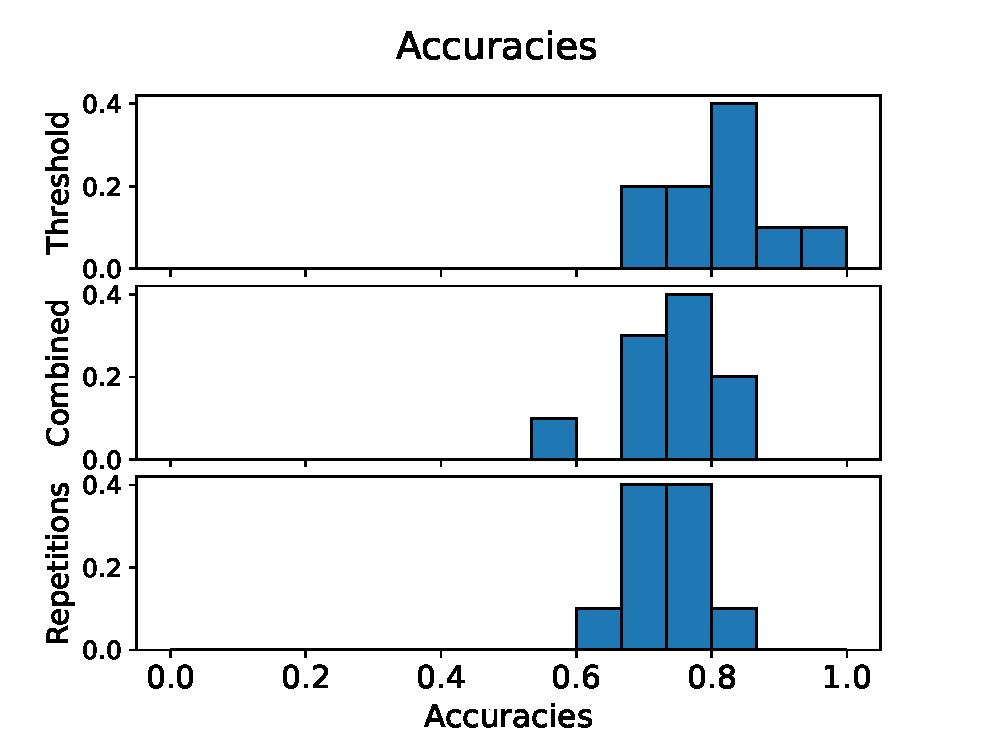
\includegraphics[width=\textwidth]{files/figs/res/trunk/acc.eps}
    \caption{}
    \label{fig:trunk-acc}
  \end{subfigure}
  ~
  \begin{subfigure}[t]{0.4\textwidth}
    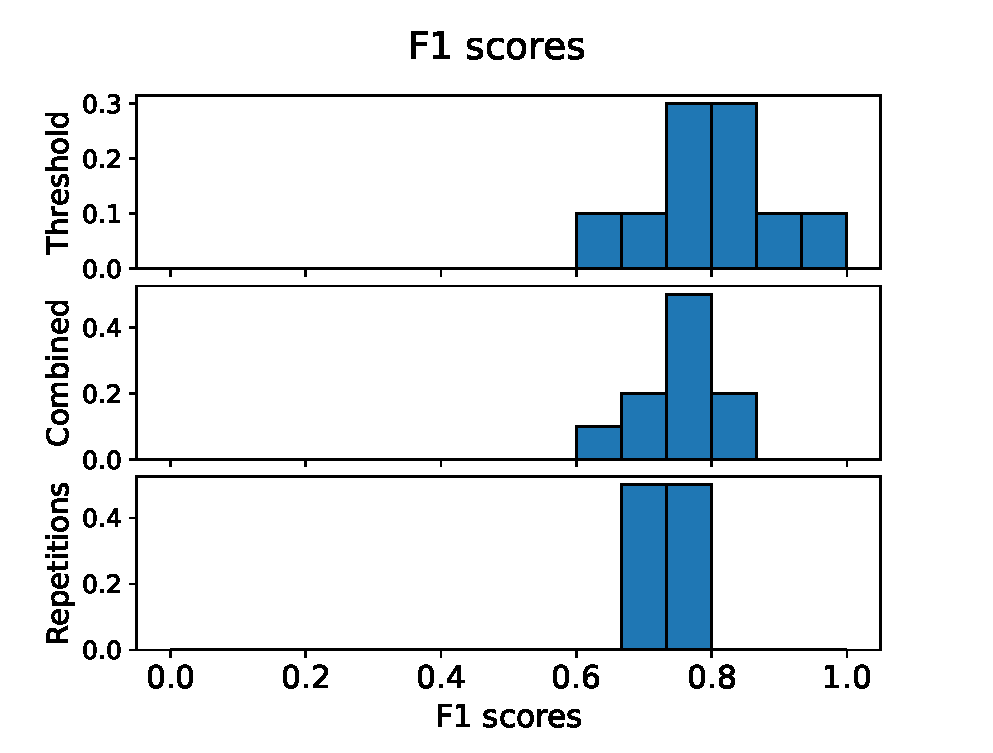
\includegraphics[width=\textwidth]{files/figs/res/trunk/f1.eps}
    \caption{}
    \label{fig:trunk-f1}
  \end{subfigure}

  \begin{subfigure}[t]{0.4\textwidth}
    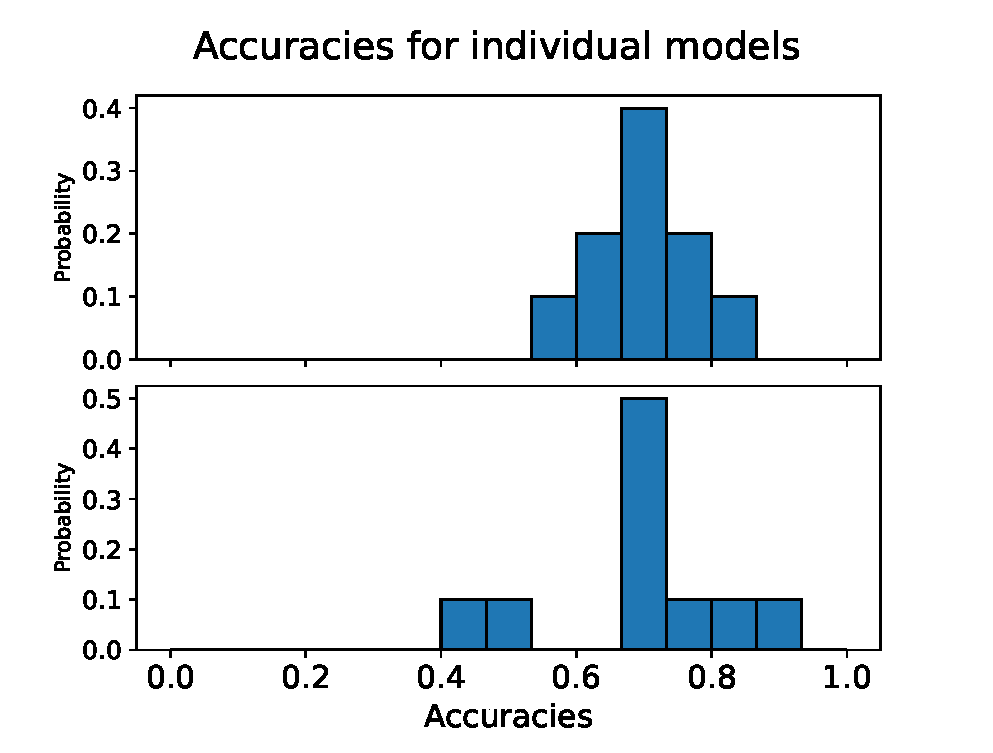
\includegraphics[width=\textwidth]{files/figs/res/trunk/acc-ind.eps}
    \caption{}
    \label{fig:trunk-acc-ind}
  \end{subfigure}
  ~
  \begin{subfigure}[t]{0.4\textwidth}
    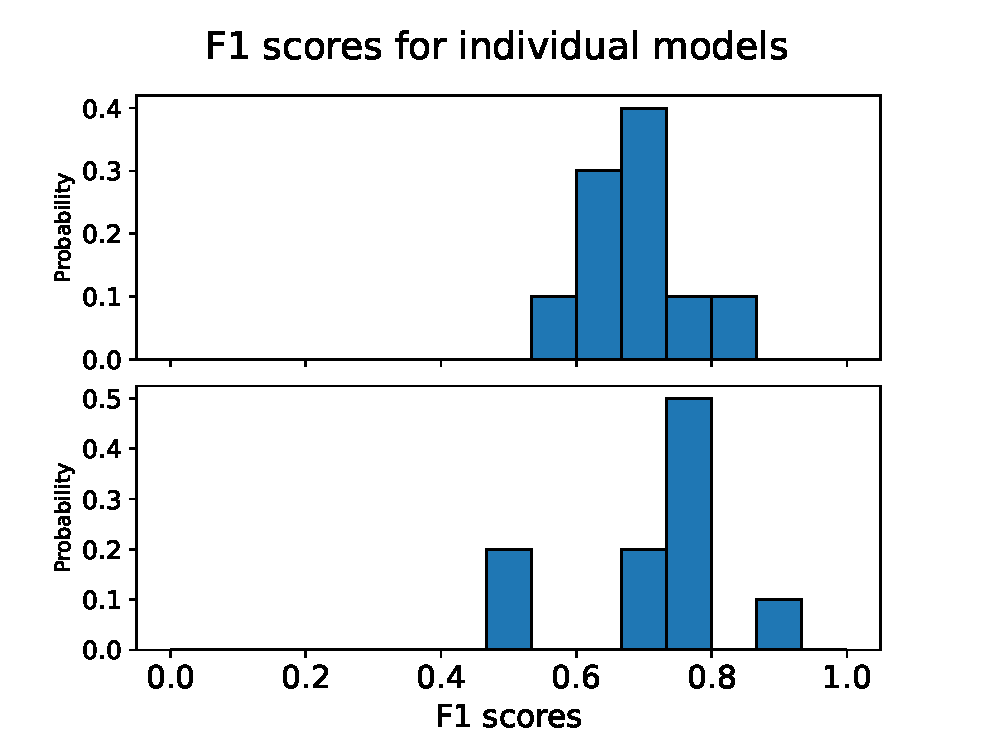
\includegraphics[width=\textwidth]{files/figs/res/trunk/f1-ind.eps}
    \caption{}
    \label{fig:trunk-f1-ind}
  \end{subfigure}
  \caption{Histograms of the accuracies and F1 scores summarized in Table \ref{tab:trunk-results} along with the same metrics for the repetition classification for the models making up the ensembles, presented in Table \ref{tab:ensemble-models}. The high precision models only predicting one class are excluded.}
  \label{fig:trunk-hist-results}
\end{figure}

Based on what is presented in Figures \ref{fig:trunk-cnfs}, \ref{fig:trunk-hist-results} and Table \ref{tab:trunk-results} it seems like the performance of the classifier is enhanced by the measures taken. Table \ref{tab:trunk-improvements} shows this is true with different confidence. Neither the combined score nor the use of an ensemble can be said to improve the performance significantly, but the combined score for the five repetitions is not primarily done to improve the performance, instead this is the way the scoring system is designed. Regarding the ensemble it might be difficult to say how big of an improvement it is based on these metrics, but it reduces the variability in the results. %As the compute increases linearly with the number of models used this becomes

\begin{table}
  \caption{With what confidence different measures led to improvements. Calculated assuming normal distributions and using pairwise comparisons for the folds. When comparing the ensemble with the individual models the best model is chosen.}
  \label{tab:trunk-improvements}
  \centering
  \begin{tabu}[c]{|c|c|c|c|}
    \hline
    & \multicolumn{1}{c|}{\begin{tabular}[c]{@{}c@{}}\textbf{Ensemble -}\\\textbf{individual} \\\textbf{models}\end{tabular}} &
    \multicolumn{1}{c|}{\begin{tabular}[c]{@{}c@{}}\textbf{Combined -}\\\textbf{Repetitions}\end{tabular}} &
    \multicolumn{1}{c|}{\begin{tabular}[c]{@{}c@{}}\textbf{Threshold -}\\\textbf{Combined}\end{tabular}} \\ \hline
    \textbf{Accuracy} & 85\% & 75\% & 99\% \\ \hline
    \textbf{F1 score} & 75\% & 85\% & 99\% \\ \hline
  \end{tabu}
\end{table}


\begin{figure}
  \centering
  \begin{subfigure}[t]{0.33\textwidth}
    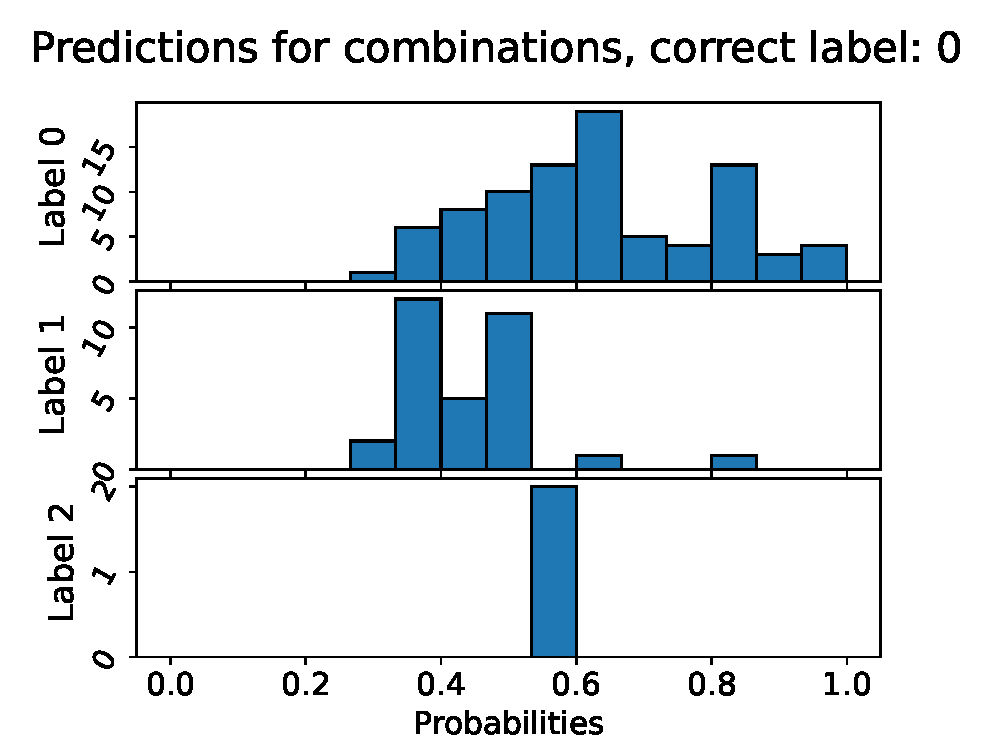
\includegraphics[width=\textwidth]{files/figs/res/trunk/pc0.eps}
    \caption{}
    \label{fig:trunk-pc0}
  \end{subfigure}%
  \begin{subfigure}[t]{0.33\textwidth}
    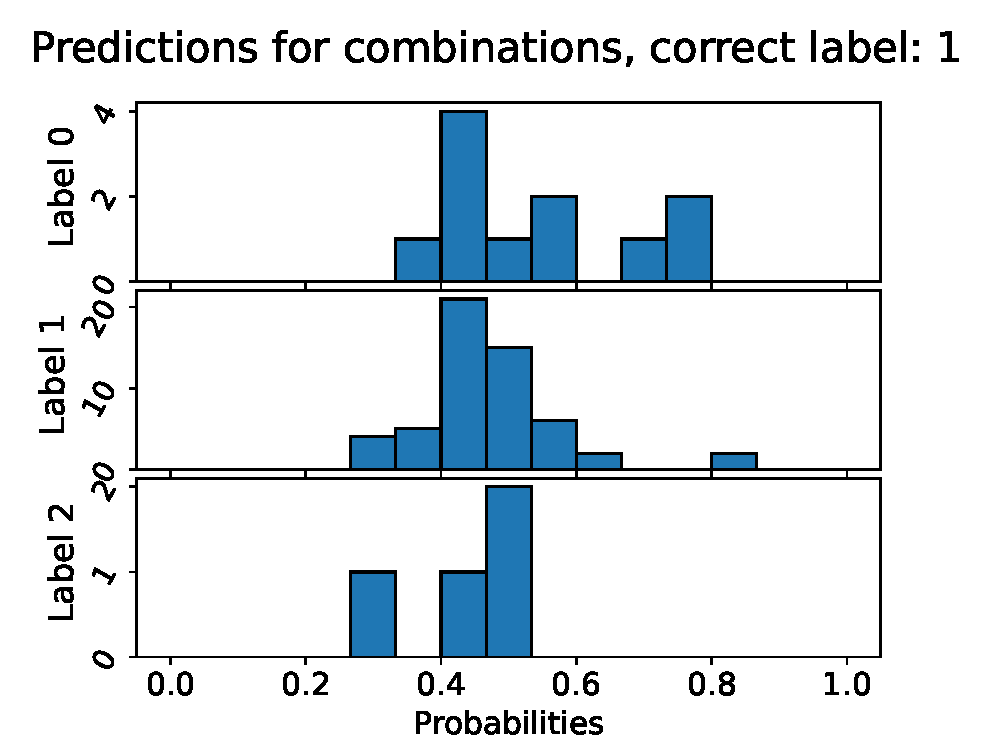
\includegraphics[width=\textwidth]{files/figs/res/trunk/pc1.eps}
    \caption{}
    \label{fig:trunk-pc1}
  \end{subfigure}%
  \begin{subfigure}[t]{0.33\textwidth}
    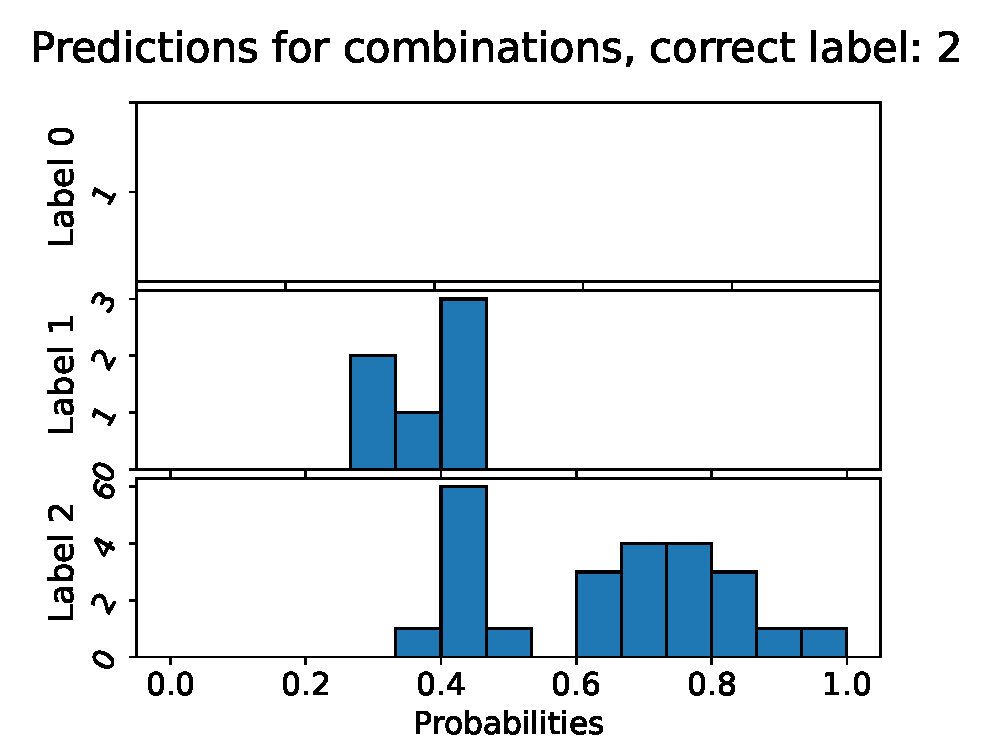
\includegraphics[width=\textwidth]{files/figs/res/trunk/pc2.eps}
    \caption{}
    \label{fig:trunk-pc2}
  \end{subfigure}

  \caption{Figures showing the probabilities for the predicted class, without threshold, for correct class 0: (a), 1: (b), 2: (c)}
  \label{fig:trunk-pc}
\end{figure}

In the results above a threshold to ignore uncertain classifications and thereby increase the performance. An extension to such a threshold, and something important for clinical use would be to provide a confidence in the classification. Figure \ref{fig:trunk-pc} shows the probabilities for the predicted class depending on which the correct class actually is. This measure seems to be rather suitable for this, with the model rarely predicting incorrectly when it outputs a high class probability. However, although the ensemble weights has been adjusted as discussed in Section \ref{sec:met-ensembles}, the probabilities for class 1 is generally low.

\FloatBarrier
